\documentclass[a4paper,toc=bibliography,headings=small]{scrbook}

\usepackage{thesis_style}
\graphicspath{{./img/}}

\setacronymstyle{long-short}
\makeglossaries
\loadglsentries{./tex/00-glossaries}

\begin{document}
\lstset{
  language=Python,
  columns=fixed,
  basewidth=0.5em,
  basicstyle=\small\ttfamily,
  numbers=left, numberstyle=\tiny\color{colorcodegray}, stepnumber=1, numbersep=5pt,
  showstringspaces=false,
  morekeywords={models, lambda, forms},
  %backgroundcolor=\color{colorbackground},   
  commentstyle=\color{colorcomments}\itshape,
  keywordstyle=\color{colorkeywords},
  stringstyle=\color{colorstrings},
  identifierstyle=\color{coloridentifiers}
}

\frontmatter
\begin{titlepage}
\begin{center}

\includegraphics[width=0.5\textwidth]{admin/uct-logo-eps-converted-to.pdf}\\[1.6cm]

{\LARGE Design and Implementation of an RFI Direction Finding System for SKA Applications}\\[1.6cm]
{\Large James Zekkai Middlemost Gowans}\\[1.6cm]

A dissertation submitted to the department of Electrical Engineering, University of Cape Town in fulfilment of the requirements for the degree of Masters of Science in Electrical Engineering\\[1.6cm]

Supervisor:\\
Prof. A. J. Wilkinson. \\[1cm]

\today

\end{center}
\end{titlepage}



% Please leave the declaration as it is (Standard UCT declaration).
\chapter*{Declaration}
\begin{enumerate}
\item I know that plagiarism is wrong. Plagiarism is to use another's work and pretend that it is one's
own.
\item I have used the IEEE convention for citation and referencing. Each contribution to, and quotation in,
this report from the work(s) of other people has been attributed, and has been cited and
referenced.
\item This report is my own work.
\item I have not allowed, and will not allow, anyone to copy my work with the intention of passing it off
as their own work or part thereof.
\end{enumerate}
\vskip 20mm
Signature:\ldots\ldots\ldots\ldots\ldots\ldots\ldots\ldots\ldots\ldots\ldots\ldots\ldots\ldots\ldots\ldots\ldots
\\J. Z. M. Gowans		% Chante this line to your name.
\vskip 20mm
Date:\ldots\ldots\ldots\ldots\ldots\ldots\ldots\ldots\ldots\ldots .


\chapter{Acknowledgments}

SKA team: Jason, Francious: resources for project, Marc: technical support for all things software related, Wes, Paul, Andrew: FPGA firmware design. Simon Norval taking me to site on two occasions to take real measurements.
SKA in general for putting up with my using their office and drinking their coffee.

Prof Inggs and Prod O'Hagan for reminding me to get on with it.

Stephen Paine for indispensable assistance in field trials and getting equipment. 

\chapter{Abstract}

Art and such.

Foobar.

\tableofcontents
%\listoffigures
%\listoftables
\printglossaries
\mainmatter
\chapter{Introduction}
\label{ch:introduction}
\section{Background}
MeerKAT is a 64-dish radio telescope aimed at being the precursor to the full \gls{ska} radio telescope. At the time of writing, the MeerKAT array is in the process of being deployed in the Northern Cape of South Africa.
MeerKAT is designed to be a highly sensitive telescope, able to detect very weak signals. It will operate over a few bands in the \SI{0.6}{\giga\hertz} to \SI{15}{\giga\hertz} range. The majority of the dishes are concentrated in the core of the array, which is set to cover an area about \SI{1}{\kilo\meter} in diameter.

Like any radio telescope, MeerKAT requires an RF-quiet environment.
The presence of \gls{rfi} on site would interfere with the ability of the telescope to collect data. At the very least, RFI would swamp the weak signals which the telescope is attempting to receive, or  worse, strong RFI could destroy the sensitive amplifiers and digitisers designed to cope only with extremely low power signals.
It is for this reason that the array is being deployed in the Karoo, away from built-up areas and the RF signals that go with such environments.

However, there is always the possibility that RFI will manifest. 
Although all equipment taken to site is tested beforehand for RFI, if equipment malfunctions or is not configured correctly or shielded correctly, RFI may be introduced. Additionally, electrical or electronic systems away from site in nearby towns or farms may inadvertently emit RFI. 
Sources such as communications systems or electronics typically emit well defined narrowband signals, while malfunctioning electronics could emit spark-like discharges producing very short bursts of broadband noise (impulsive RFI).
As such, RFI management systems must be in place to aid in the detection and amelioration of RFI in order to allow the telescope to function optimally. 

In Electronic Warfare, \gls{aoa} is a critical useful parameter in hostile emitter sorting as it cannot be varied by the emitter \cite{center2012electronic}.The purpose of this research is to design a device capable of detecting RFI and performing \gls{aoa} parameter estimation on the detected signals.
The process of estimating the \gls{aoa} of a signal is known as \gls{df}.
Knowing the \gls{aoa} will allow the SKA team to track down where rogue RFI signals are coming from and to silence them.

\begin{figure}[hb]
  \centering
  \includegraphics[width=0.71\textwidth]{introduction/meerkat-array}
  \includegraphics[width=0.25\textwidth]{introduction/meerkat_dish}
  \caption{Photo of the MeerKAT core and a close up of an antenna. Src: \cite{skasawebsite}}
\end{figure}

\section{User Requirements}

The following user requirements were drawn up by three senior engineers at SKA SA: the Director of Science and Engineering, Prof Justin Jonas, Systems Engineer for Infrastructure, Carel van der Merwe and digital backend DSP specialist, Dr Jason Manley. 

\begin{enumerate}
  \item A system to perform direction finding of both impulsive and continuous wave (CW) RFI sources is to be designed.
  \item They key deliverables of this project are a software package and a thesis report.
  \item The software package should have the following functions:
    \begin{enumerate}
      \item It should take in input from a correlator. This could either be time domain cross correlation for impulsive sources or frequency domain cross correlation for continuous sources. 
      \item It should parse a configuration file which contains information about the array configuration and information about the output from the correlator.
      \item The data from the correlator should be used to ascertain the direction of the detected signals.
      \item The software should be designed to fit into a system which has a 100\% \gls{poi}
    \end{enumerate}
  \item The software should have the following user interface features:
    \begin{enumerate}
      \item The user should connect to it via a web interface.
      \item A streaming waterfall plot of frequency vs amplitude should be displayed to the user to serve as monitoring of the RFI environment.
      \item The user should be able to select a band of interest from the waterfall plot.
      \item The direction finding should then be computed for the signal in that band.
      \item The result of the DF should be presented to the user. An investigation must be done into the best way to present this information to the user.
      \item Where appropriate, additional meta information should be displayed to the user, such as measurement accuracy or signal strength.
    \end{enumerate}
  \item The system should be designed to find terrestrial RFI sources.
  \item The system should be designed to be location independent. It could either be deployed to a fixed location or as a mobile device deployed on a vehicle.
  \item This project should be able to interface easily with other systems requiring its data. Specifically, it should be designed to interface with and pass its data on to an allied project which is doing classification of RFI.
  \item The system should be real-time, where real-time is defined as having a latency in the order of a few seconds from receiving signals to displaying results to the user. 
  \item The hardware and software used should be in line with what is used at MeerKAT. This implies the ROACH platform for hardware, Python for back end software and JavaScript for front end software.  
  \item This system must operate in the context of the MeerKAT site, implying the following:
  \begin{enumerate}
      \item In general, the RF environment is sparse. While there will be multiple simultaneous transmitters, it can be assumed there will only be one transmitter in a channel and one source of transients at a given time.
      \item The sources of the emissions will be relatively slow moving, up to the maximum speed of a vehicle on a dirt road; \SI[per-mode=symbol]{60}{\kilo\metre\per\hour}.
  \end{enumerate}

  \item Once the software has been completed, its performance on real life data should be quantified in the following way:
    \begin{enumerate}
      \item A prototype-stage 4-element antenna array should be connected to a \SI{400}{\mega\hertz} baseband digitiser and correlator.
      \item The correlator need not be real time for the demonstration.
      \item As the goal of this project is not to develop a hardware system, there is no specific requirement on receiver sensitivity or noise figure. Whatever the best available hardware is should be used for the antennas, front end and digitiser. 
      \item The performance of the hardware used should be analysed. 
    \end{enumerate}
  \item Mitigation of the effects of performance degradation due to multipath is outside of the scope of this work.

  \item The report produced should contain a theoretical analysis of the performance of the system, as well as an analysis of the performance of the prototype on site with real signals. 
\end{enumerate}

\section{Requirements Review}
The requirements as stated by the \gls{ska} are clear and understood. Some notable implications from the requirements:

\begin{itemize}
  \item The system which will be designed here will probably not be immediately applicable to combating RFI at the MeerKAT site. The reason is that this project is focused on the \gls{df} implementation, not hardware. Hence no down converter will be designed in meaning the frequency band being digitised by this system will not overlap the MeerKAT band. 
    It will be up to future work to add a suitable \gls{rf} front end in order to allow the system to operate in the MeerKAT band of interest. However, the implication for this work is that it is essential that this system be designed such that it is trivial to reconfigure the system for a different RF front end and frequency band. 

  \item Based on the fact that the emitters will be either stationary or slow moving, it should be acceptable to have integration times in the order of 1 second. 

  \item The requirement of a 100\% \gls{poi} will impose restrictions on what antenna array and receiver can be used, and this will in turn have restrictions on the specific \gls{df} algorithm which can be used. 

  \item Seeing as this system is intended to be used by \gls{ska} and will require future work to make it production ready, the source code should be structured such to allow collaborative development and located somewhere accessible. Github will be used. Following is a list of code repos used in this project. 

\end{itemize}

\begin{table}
  \centering
  \begin{tabu}{c|c}
    Description & URL \\
    \hline
    This document & \url{https://github.com/jgowans/masters_writeup} \\
    Ambiguity simulation & \url{https://github.com/jgowans/phase_ambiguity} \\
    iADC calibration & \url{https://github.com/jgowans/iADC_calibration} \\
    Direction finder front end & \url{https://github.com/jgowans/directionFinder_web} \\
    ROACH firmware & \url{https://github.com/jgowans/correlation_plotter} \\
    Direction finder backend & \url{https://github.com/jgowans/directionFinder_backend} \\
  \end{tabu}
  \caption{Github repos for this project}
  \label{tab:lit-review-repos}
\end{table}

\section{Report Outline}
This, Chapter 1, has contained the problem statement and user requirements of the system which needs to be designed an implemented. 

Next in \Cref{ch:lit-review}, the existing literature around DF systems will be explored. This will serve as the foundation for the system being designed here. The exploration will focus on direction finding fundamentals and a comparison of algorithms. It will examine DF for both continuous narrow band signals and impulsive signals. It will explore detection algorithms for impulsive sources, as well as calibration techniques and error calculations. The outcome of this chapter should be sufficient information to make informed system design decision.

\Cref{ch:system-design} contains the high level system design, showing what blocks need to be designed and how they will be linked together in order to build a complete system. Here, the system is broken into three main components: the RF front end, the ROACH digitiser and DSP engine, and computer software for final AoA computation and logging. Additionally, the exactly DF algorithm being used by the system will be defined and simulations of its performance run.

\Cref{ch:rf-front-end} discussed the antenna array and RF front end. It details designing and building the 4-element antenna array, as well as assembling and measuring a board of low noise amplifiers and filters.

\Cref{ch:firmware-design} discusses the implementation of the FPGA firmware to do data acquisition and the first stage of DSP. The focus is on designing the FPGA sub-system in simulink and demonstrating it being functional both in simulink simulations and, most importantly, running on hardware and processing real signals in the lab.

\Cref{ch:software-design} details Python code which implements the direction finding algorithms. It requires interfacing the computer with the ROACH to read out data, creating a model of the antenna array, and estimating the AoA based on the received data and the array model. It also has to handle calibration, logging, and showing signal plots to give the operator insight into the signals being received.

\Cref{ch:field-trials} reports on the field trials of the DF system. There are two field trials sessions: one early in the project with a basic system, to get a feel for the types of RFI data. Another with the final system doing real DF measurements and checking the accuracy of the system.

\Cref{ch:conclusions} contains conclusions indicating what has been achieved in the project and comments on the system which has been implemented. Also, scope for future work is looked at.


\chapter{Literature Review}
\label{ch:lit-review}
In this chapter an exploration of the current literature around direction finding is undertaken.
It will first cover an overview of the fundamentals of antenna arrays and signals in order to establish the concepts, terminology and mathematics required to understand specific DF techniques. 
Next, a variety of DF techniques will be analysed. The algorithm and principal of each technique will be presented, followed by the advantages and disadvantages of the technique. 
These advantages/disadvantages will be tied back to the user requirements defined in \Cref{ch:introduction} to ascertain whether the technique is appropriate for this application. Where possible, existing systems which implement a particular technique will be cited as examples.

The purpose of this chapter is to gain sufficient information about the various DF techniques to make informed system design decisions in \Cref{ch:system-design}, as well as to implement accurate simulations.

\subsection{Radio Frequency Signals and Antennas}
Some RF fundamentls used for modelling.

\section{Model from electronic warfare target location method}

The model which will be discussed here is that presented in \cite{poisel2012electronic}.  

Let there be an array of $M$ antenna elements receiving signals, where the position of of the \(m\)th element is \(\vec{x}_{m} = \begin{bmatrix}x_m & y_m & z_m \end{bmatrix}\).
The signal received by this \(m\)th element is influenced by the element position. 
This can be represented as \(\vec{r}_m(t, \vec{x}_m)\), showing that the signal at the \(m\)th element is a function of the position of the element.
As discussed by \cite{krim1996two}, this model contains both spacial and temporal information and hence is sufficient to be able to attain spacial information about the signal. 

It is further shown by Poisel that the delay time for a signal arriving at the \(m\)th sensor from a source located at azimuth angle \(\theta\) and elevation angle \(\phi\) is
\begin{align}
 \tau_m(\vec{\theta}) &= \tau_m ( \begin{bmatrix} \theta \\ \phi \end{bmatrix} ) \\
                       &= \frac{1}{c} [ x_m\cos(\theta)\cos(\phi) + y_m\sin(\theta)\cos(\phi) + z_m\sin(\phi) ]
\end{align}
This model assumes that the azimuth and elevation angle to the source, \(\begin{bmatrix}\theta & \phi\end{bmatrix}\TRANSPOSE\), is the same for each sensor. This is approximately true when the distance from the array to the source is much greater than the array geometry. Hence, it's often convenient and most accurate to select the center of the array as the origin. 
For a 2D space we let \(\phi = 0\) and hence simplify to:
\begin{equation}
 \tau_m(\theta) = \frac{1}{c} [ x_m\cos(\theta) + y_m\sin(\theta) ]
\end{equation}
Expressed as a matrix multiply:
\begin{align}
\tau_m(\theta) &= \frac{1}{c}\begin{bmatrix}x_m & y_m\end{bmatrix}\begin{bmatrix}\cos\theta\\ \sin\theta\end{bmatrix} \\
          &= \frac{1}{c} \vec{x}_m \vec{k}(\theta)
\end{align}
Where \(\vec{k}(\theta) = \begin{bmatrix}\cos\theta& \sin\theta\end{bmatrix}\TRANSPOSE\) is the wavenumber vector which graphically equates to the 'ratio' of how much the signal propagates in the x direction per distance propagated in the y direction. It's not really a ratio, it's a vector, so this doesn't quite makes sense. Note to self: tidy this up.

If this time delay is multiplied by the frequency in radians per second, \(\omega\), the result is the phase difference at the element relative to the origin:
\begin{align}
  \phi_m(\theta, \omega) &= \omega\tau_m(\theta) \\
                         &= \frac{\omega \vec{x}_m \vec{k}(\theta)}{c} \\
                         &= \frac{ \vec{x}_m \vec{k}(\theta) }{\lambda}
\end{align}

Representing the phase shift of all M sensors as a vector,
\begin{equation}
  \vec{\phi}(\theta, \omega) = \frac{\mathbf{X}\vec{k}(\theta)}{\lambda}
\end{equation}
Where \(\mathbf{X}\) is a \((M \times 2)\) matrix containing the \(x\) and \(y\) coordinates of each of the M sensors. 
In general, the output of an array is also impacted by the amplitude scaling and phase shifting applied to the received signals by the beam pattern of each sensor. The combination of the phase shift resulting from the physical separation of the sensors and the amplitude/phase response of a sensor is a very key property of an array known as the antenna array manifold, or steering vector, or source-position vector:
\begin{equation}
  \boxed{
    \vec{a}(\theta, \omega) = \vec{g}(\theta, \omega) \odot \exp \left\{ j \frac{\omega \mathbf{X} \vec{k}(\theta)}{c} \right\}
  }
\end{equation}

Often (as is the case in this project) the sensors used will be identical omnidirectional antennas. In this case, the amplitude and phase shift of the antennas as a result can be ignored, as it will be equal between elements and independent of angle or arrival. 
\begin{equation}
  \vec{a}(\theta, \omega) = \exp \left\{ j \frac{\omega \mathbf{X} \vec{k}(\theta)}{c} \right\}
\end{equation}

Or, more verbose:
\begin{align}
\vec{a}(\theta, \omega) &= \exp \left\{ \frac{j \omega}{c} \begin{bmatrix} x_1, y_1 \\ x_2, y_2 \\ .., .. \\ x_M, y_M \end{bmatrix} \begin{bmatrix} \cos(\theta) \\ \sin(\theta) \end{bmatrix} \right\} \\
                        &= \exp \left\{ \frac{j \omega}{c} \begin{bmatrix} x_1\cos(\theta) + y_1\sin(\theta) \\ x_2\cos(\theta) + y_2\sin(\theta)) \\ .., .. \\ x_M\cos(\theta) + y_M\sin(\theta) \end{bmatrix} \right\} \\
\end{align}

The vector output of the array, \(\vec{r}(t)\), where each element of the vector is the signal received by the sensor is the where each element of the vector corresponds to an antenna element is equal to the sum of the signals at that element by the principle of superposition. Algebraically:
\begin{equation}
  \vec{r}(t) = \sum_{k=1}^{K} s_k(t)\vec{a}_k(\vec{\theta}_k) + \vec{n}(t)
\end{equation}
Where:
\begin{itemize}
  \item \(s_k(t)\) is the source signal,
  \item \(\vec{\theta}_k = \begin{bmatrix} \phi_k, \theta_k \end{bmatrix}\TRANSPOSE\) is the source parameter vector, a vector with azimuth and elevation angles pointing in the direction of the source,
  \item \(\vec{a}_k(\vec{\theta}_k)\) is the antenna array manifold, explored more shortly,
  \item \(\vec{n}(t)\) is additive noise.
\end{itemize}

Or in matrix notation:
\begin{align}
  \vec{r}(t) = \mathbf{A}(\vec{\theta})\vec{s}(t) + \vec{n}(t)
\end{align}

The array manifold vector is also known as source position vector or as the steering vector. It is the response of the array to a signal impinging on the array from a certain azimuth and elevation angle, \((\phi, \theta)\). The response is naturally in terms of the gain and phase shifts introduced by each sensor as a result of the beam pattern and physical separation of the sensors. It is given by:
\cite{dacos1995estimating}.
\begin{equation}
\vec{a}(\theta, \phi) = \vec{g}(\theta, \phi) \odot \exp \left\{ -j \mathbf{X}\TRANSPOSE \vec{k}(\theta,\phi) \right\}
\end{equation}
Where:
\begin{itemize}
  \item \(\vec{g}(\theta, \phi)\) is a \(N\)-dimensional vector of complex number being the gain and phase response  of each element in the direction \((\theta, \phi)\). 
\item \(\mathbf{X}\TRANSPOSE\) is a \((N \times 3)\) matrix containing the \(x\), \(y\) and \(z\) coordinates of each of the N elements of the form \(\begin{bmatrix} \vec{x}, \vec{y}, \vec{z} \end{bmatrix}\TRANSPOSE\)
\item \(\vec{k}(\theta, \phi)\) is the wavenumber vector given by \(\vec{k}(\theta, \phi) = \pi \begin{bmatrix} \cos\theta\cos\phi, \sin\theta\cos\phi, \sin\phi \end{bmatrix}\TRANSPOSE \). Graphically, this equates to the 
\end{itemize}
For the purposes of this research the elements will all be located at the same elevation as we only with to locate terrestrial signals. Hence, this may be simplified to:
\begin{equation}
  \vec{a}(\theta) = \vec{g}(\theta) \odot \exp \left\{ -j \mathbf{X}\TRANSPOSE \vec{k}(\theta) \right\}
\end{equation}
Here, \(\mathbf{X}\TRANSPOSE\) is now a \((N \times 2)\) matrix of the form \(\begin{bmatrix} \vec{x}, \vec{y} \end{bmatrix}\) and \(\vec{k}(\theta) = \pi[\cos(\theta), \sin(\theta)]\TRANSPOSE\).

Furthermore, the \(\vec{g}\) term may be excluded if we assume omnidirectional elements. Although it is rare to deal with true omnidirectional antennas, for an antenna which is required to receive signals only in the azimuth plane, omnidirectional antennas such as dipoles might very well be used in practice. This hence simplifies to:

\begin{equation}
  \vec{a}(\theta) = \exp \left\{ -j \mathbf{X}\TRANSPOSE \vec{k}(\theta) \right\}
\end{equation}



The antenna array manifold can now be re-written:
\begin{align}
\vec{a}(\theta) &= 
  \exp \left\{ -j \begin{bmatrix} 
      \omega_c \tau_1(\phi_k)\\ 
      \omega_c \tau_2(\phi_k)\\ 
      \omega_c \tau_M(\phi_k) 
   \end{bmatrix} \right\} \\
  &= \begin{bmatrix}
      e^{-j\omega_c \tau_1(\phi_k)} \\
      e^{-j\omega_c \tau_2(\phi_k)} \\
      ... \\
      e^{-j\omega_c \tau_M(\phi_k)} \\
   \end{bmatrix}
\end{align}

Clearly, this is simply a vector of phase shifts introduced by each element in the array as a function of both the location of the element and the angle of the incident wave relative to some defined zero location and zero direction. It is said by \cite{dacos1995estimating} that this array manifold completely characterises the array. That paper goes into additional details on how the manifold may simplified for linear arrays, as well as the special properties which a manifold of a linear array possesses. This will not be discussed here as the array used for this DF system is not likely to be linear. 

Let there be $K$ individual signal sources, where $\vec{s}(t)$ represents the resultant signal, being
\begin{equation}
\vec{s}(t) = \begin{bmatrix} s_{1}(t) & s_{2}(t) & s_3(t) & ... & s_K(t) \end{bmatrix}
\end{equation}

This important result shows us that for a known array with omnidirectional antennas at arbitrary \(x)\) and \(y\) locations, receiving a narrow band signal of known frequency from a certain direction, \(\theta\), the phase shift at each element is a vector which can be easily calculated. This is the basis around which the direction finding algorithm for this project will be designed. 

\section{Direction Finding Techniques}
A direction finder is a passive device able to ascertain the angle of arrival of a source of electromagnetic radiation.
The objective of direction finding is generally to find the location of non-cooperative emitters\cite{poisel2012electronic}.
This is one of the fundamental activities of electronic defense as well as RFI hunting.
The general structure of a direction finding system is an antenna array connected to a receiver connected to a processing module connected to a display providing output to operators.
Simple direction finding systems were used as early as the start of the \nth{20} century and have been continually evolving since then along with developments in communications and electronic warfare systems.
Direction finding systems have applications in a variety of applications, ranging from radar, sonar, surveillance, radio astronomy and even medical. Finding an optimal parameter estimator for angle of arrival is difficult and hence lots of research has been done into the topic over the last few decades\cite{van2004detection}.

DF techniques are generally based on either amplitude comparison, time/phase comparison or statistical methods\cite{tuncer2009classical}. 
Various implementations of these classes of DF will now be explored.

Much of following overview of types of direction finding systems is based on discussions in the Electronic Warfare and Radar Systems Engineering Handbook\cite{center2012electronic}.

\subsection{Scanned beam}
This is a direct amplitude technique. An antenna with gain (non-uniform beam) is rotated and this causes the power output of the antenna to vary with rotation angle. This is the earliest form of direction radio direction finding and was implemented in the early 1900's. 
One of the first uses of this DF technique was in a system developed by Marconi to locate the bearing to a ship which was transmitting a signal for navigation purposes\cite{jenkins1991smallaperture}. A loop antenna was frequently used as it was a simple antenna to construct and the beam pattern has a sharp null. 
An example antenna and beam pattern are shown in \Cref{fig:lit_loop_antenna}. As the change in antenna output power per degree rotated is highest around the null, the antenna was often aligned such that the signal of interest was in the null. 
If multiple signals originating from different bearings are present, the system cannot operate. 
While today it may be possible to put highly selective receivers on the output of the antenna, this technology did not exist when scanning beam DF systems were originally used.

Note that as the beam pattern is symmetric about both the \(x\) and \(y\) axis, there are in general 4 ambiguous points. However, if the antenna can be rotated such that the signal is in the null, there is then only 2 ambiguous points, or \SI{180}{\degree} ambiguity. This ambiguity can be resolved with an  additional antenna element. Note also that this is not an instantaneous DF technique as it requires time for the antenna to be rotated. Hence, this technique is not suitable for finding transients. 

Loop antennas DF systems are very sensitive to multipath errors, especially ionospheric reflection \cite{jenkins1991smallaperture}. 
\begin{figure}
  \centering
  \begin{subfigure}[b]{0.48\textwidth}
    \centering
    \includegraphics[width=0.8\textwidth]{lit_review/loop_antenna}
    \caption{Loop antenna used for direction finding in 1918. Src: \cite{grabau1989funkpeiltechnik}}
  \end{subfigure}
  ~
  \begin{subfigure}[b]{0.48\textwidth}
    \centering
   \includegraphics[width=0.7\textwidth]{lit_review/loop_antenna_beam}
   \caption{Beam pattern of loop antenna or dipole. Note the sharp null. Src: \cite{jenkins1991smallaperture}}
  \end{subfigure}
  \caption{Loop antenna and beam pattern}
  \label{fig:lit_loop_antenna}
\end{figure}

\subsection{Crossed Loop}
The crossed loop technique is an amplitude comparison technique. 
As is shown in \Cref{fig:lit_crossed_loop_antenna}, using two loop antennas perpendicular to one another produces two beam patterns: one being proportional to the sine of the angle and the other to the cos of the angle. 
By comparing the signal power from each antenna, it is possible to ascertain the \gls{aoa}. This system is instantaneous as only a single pulse is necessary to ascertain the ratio of antenna output power. However it has many ambiguities. Some ambiguities can be resolved with a sense antenna. 
For optimal ambiguity resolution, the crossed loop should be rotated such that signal of interest is located in the null of one of the loops and the peak of the other. This resolves ambiguity but at the expense of the system not being real-time.
As with the scanned beam, the crossed loop suffers from significant performance degradation arising from multipath, specifically ionospheric reflection. 
In the 1930's a marine radio direction finder network using the crossed loop amplitude comparison technique was set up for marine navigation. Then, during World War II, rapid improvements to DF technology were made with the operating frequency of the systems being extended into the VHF and UHF band  and extensive DF networks being installed\cite{jenkins1991smallaperture}. The tactical advantage which DF systems provided prompted significant development into DF during the war.
\begin{figure}
  \centering
  \begin{subfigure}[b]{0.3\textwidth}
    \includegraphics[width=\textwidth]{./img/lit_review/loop_antenna_crossed}
    \caption{Example of crossed loop antenna.}
  \end{subfigure}
  ~
  \begin{subfigure}[b]{0.4\textwidth}
    \includegraphics[width=\textwidth]{./img/lit_review/loop_antenna_crossed_beam}
    \caption{Crossed loop antenna beam pattern showing difference in magnitude seen by each loop. Src: \cite{jenkins1991smallaperture}}
  \end{subfigure}
  \caption{Crossed loop antenna and beam pattern}
  \label{fig:lit_crossed_loop_antenna}
\end{figure}

\subsection{Adcock Array}
The Adcock array was developed and patented in 1919 by British army engineer Frank Adcock \cite{gething1991radio}.
Instead of using loop antennas, the Adcock array makes use of two orthogonally orientated (crossed) pairs of monopole or dipole antennas. Typically a North-South pair and an East-West pair are used. These antenna pairs produce the same beam pattern as the loop antennas. 
As a loop antenna can be modeled by two vertical antennas on the sides and two horizontal antennas on the top and bottom of the loop, it should be clear that the loop is not polarisation selective. While the direct beam from the signal source may be vertically polarised, the reflected beam from atmospheric reflection was also being received and corrupting the signal output of the array.
The Adcock array which uses only vertical elements maintains the same beam pattern as the loop but is not sensitive to horizontally polarised radiation hence offers better performance for a DF system.
The antenna configuration of Adcock and Watson-Watt is shown in \Cref{fig:lit_adcock_array}.
This array configuration was studied extensively in the 1930's and played a significant role in the electronic warefare of World War II \cite{gething1991radio}. One of the advantages of it at the time was that the output it provided allowed it to directly drive a CRT display, giving the user real-time visibility into what the system was receiving\cite{jenkins1991smallaperture}. 

\begin{figure}
  \centering
  \begin{subfigure}[b]{0.25\textwidth}
    \includegraphics[width=\textwidth]{./img/lit_review/adcock_model}
  \end{subfigure}
  ~
  \begin{subfigure}[b]{0.6\textwidth}
    \includegraphics[width=\textwidth]{./img/lit_review/adcock_implementation}
  \end{subfigure}
  \caption{Left: model for adcock antenna showing N-S and E-W pairs. Right: Japanese implementation of array for 2 MHz direction finding. Src: \cite{japanesecommunications}}
  \label{fig:lit_adcock_array}
\end{figure}


\subsection{Watson-Watt Evaluation}
This amplitude comparison technique is probably the most commonly used DF technique over the history of DF systems\cite{poisel2012electronic}.

Ambiguity and multipath are one of the major difficulties which need to be overcome in direction finding systems. 
In the mid 1920s, Sir Robert Watson-Wat developed an improved DF system based on the Adcock array configuration. 
As discussed above, the beam pattern of the output of an Adcock array is one cosine shaped beam and one sine shaped beam. By exploiting the trigonometric properties of these functions and adding an additional sense element, Watson-Watt developed a method to compute the angle of arrival from an array with this cos/sin property. 
This evaluation technique showed significant improvement in rejection of ionospheric reflections and made ambiguity resolution easier.
In the case of Wattson-Watt, the beams are synthesised by forming sum and difference channels from broad beam antennas in an array.

The mathematics around this technique will not be explored in detail here, but a graphical view of the antenna and receiver structure can be seen in \Cref{fig:watson-watt}.
For a more detailed discussion of the mathematics behind the Watson-Watt DF algorithm, see Poisel\cite{poisel2008introduction}.
For a simulation of Watson-Watt algorithm as well as a discussion around an ambiguity resolution implementation using a sense antenna see Pellejero\cite{adcockwatsonwattrdf}.

\begin{figure}
  \centering
  \begin{subfigure}[b]{0.48\textwidth}
    \includegraphics[width=\textwidth]{./img/lit_review/watson-watt-processing-analogue}
    \caption{View showing transformer configuration to produced required difference signals. Src: \cite{poisel2008introduction}}
  \end{subfigure}
  ~
  \begin{subfigure}[b]{0.48\textwidth}
    \includegraphics[width=\textwidth]{./img/lit_review/watson-watt-processing-digital}
    \caption{Abstraced view of signal chain for digital processing. Src: \cite{rhode2000introtodf}}
  \end{subfigure}
  \caption{Watson-Watt array processing technique using the Adcock array. Note that difference channels from crossed beams are formed}
  \label{fig:watson-watt}
\end{figure}

\subsection{Doppler}
By the principle of Doppler shift, moving an antenna towards a signal source increases the observed frequency while moving an antenna away from a source lowers the observed frequency. 
If an antenna is rotated around a central point (tracing out the circumference of a circle), there will be 
The Doppler shift is given by: \cite{poisel2012electronic}
\begin{equation}
  \Delta f = \frac{B\omega}{c}f_c\sin(\Uppsi)
\end{equation}
Where \(B\) is the length of the antenna baseline, \(\omega\) is the angular velocity of the antenna, \(f_c\) is the carrier frequency of the signal source and \(\Uppsi\) is instantaneous difference between the angle towards the signal source and the angle of the rotating antenna (this is shown graphically in \Cref{fig:lit-review-doppler-switching}). By rotating one antenna around a reference antenna and measuring the received signal frequency difference, the Doppler shift can be measured and with the above equation the AoA calculated.

However, to DF a \SI{100}{\mega\hertz} tone with a Doppler shift of \SI{3}{\mega\hertz}, the antenna would need to be rotated with a tangential velocity of 10000 m/s\cite{jenkins1991smallaperture}. 
It is not practical to rotate an antenna at such a high speed. 
Hence, rather than physically rotating an antenna, what is done in practice is that a Doppler shift is synthesised by rapidly switching between sampling different elements of a large circular array. 
Typically between 12 and 30 elements are used for Doppler DF arrays. 
\Cref{fig:lit-review-doppler-switching} shows a typical implementation of a Doppler DF system using antenna switching.

As discussed by Jenkins \cite{jenkins1991smallaperture}, Doppler is not a high accuracy system due to the signal distortion introduced by switching the sampled antenna. Furthermore, Doppler DF is not suited to locating transients for two reasons:
\begin{enumerate}
  \item it is not an instantaneous technique due to there being some time required to switch between sampling all of the antennas. For example, a typically time required to switch between all elements of an array may be \SI{6}{\milli\second} \cite{rhode2000introtodf}. This is unsuitable for transients which may last only a few hundred nanoseconds.
  \item it generally needs a narrow-band signal which has a well defined carrier frequency so that the Doppler shift is well defined. Impulsive transients do not have this characteristic.
\end{enumerate}

For a more detailed discussion of the mathematics behind Doppler DF, see the Rhode \& Schwarz report \cite{rhode2000introtodf}. 
\begin{figure}
  \centering
  \begin{subfigure}[b]{0.48\textwidth}
    \centering
    \includegraphics[width=\textwidth]{./img/lit_review/doppler-2-antenna}
    ~ 
    \caption{Model for Antenna 2 rotating around stationary Antenna 1 with angular velocity \(\omega\). Src: \cite{poisel2012electronic}}
  \end{subfigure}
  ~
  \begin{subfigure}[b]{0.48\textwidth}
    \centering
    \includegraphics[width=0.6\textwidth]{./img/lit_review/doppler-switching}
    \caption{Practical implementation switching antennas for pseudo-Doppler DF system. Src: \cite{jenkins1991smallaperture}}
  \end{subfigure}
  \caption{Model for Doppler DF system}
  \label{fig:lit-review-doppler-switching}
\end{figure}


\subsection{Time Difference of Arrival}
\gls{tdoa} is a DF system which is typically used for finding of impulsive sources; sources which emit a pulse that exists for a short time duration where the pulse has a clearly defined start and end. Most commonly it is used for locating pulsed radar system in the electronic warfare context.

For a two element array, the difference in time, \(\delta t\) in the arrival of a pulse at the elements is
\begin{equation}
  \delta t = \frac{d \cos \theta}{c}
\end{equation}
Where \(d\) is the element spacing, \(\theta\) is the AoA and \(c\) is the speed of light.

This technique requires the ability to measure the start of a pulse very accurately, or alternatively to be able to measure the difference very accurately through cross correlation. Additionally, it requires a comparatively large SNR. The primary advantage of it are that it is independent of frequency and does not suffer from ambiguity when receiving impulsive signals\cite{jenkins1991smallaperture}.

\subsection{Phase Interferometry}
This technique is done by comparing the phase arriving at each element of an array.
In general, it is a higher complexity technique and may suffer from ambiguity, but it can achieve comparatively high accuracy direction measurements, often between \SI{0.1}{\degree} and \SI{3}{\degree} for real systems\cite{center2012electronic}.
In comparison to amplitude systems, phase systems are more tolerant of multipath signals. 
The high complexity is introduced due to needing to perform real-time high accuracy phase measurements of the signals at multiple antennas and having to incorporate ambiguity resolution algorithms.
Also, they often impose stringent requirements on the phase matching for the RF chain which requires careful design, measurement and calibration\cite{schleher1999electronic}.

The simplest phase interferometry system is a two element array. This is shown graphically in \Cref{fig:lit-two-element-phase} where \(d\) is the element spacing, \(\lambda\) is the wavelength and \(\theta\) is the AoA or difference between the boresight and wavevector.
The phase difference at the output of the system is calculated as follows:
\begin{equation}
\phi = \frac{2 \pi d \sin \theta}{\lambda}
\end{equation}
Notes about this simple two element array:
\begin{enumerate}
  \item The values of the sine function of only unique between \SI{-90}{\degree} and \SI{90}{\degree}. Hence, the output of the array is only unambiguous over this \SI{180}{\degree} field of view. A two element phased interferometry array cannot resolve this ambiguity. The best it can do is use antennas with gain to reject signals from outside of its field of view.
  \item If the element spacing is larger than \(\frac{\lambda}{2}\) (as shown in the figure) the ambiguity gets worse. The unambiguous field of view for a 2-element array is: \(\theta_{FOV} = 2 \sin^{-1}(\frac{\pi}{2d})\). Clearly, as \(d\) gets larger \(\theta_{FOV}\) gets smaller. 
  \item Although ambiguity gets worse with a larger spacing, angular accuracy improves. This is because the system has a percentage RMS error and when the FOV is shrunk, the error in degrees (which is a percentage of the FOV) also decreases. Hence, there is a trade-off between ambiguity and accuracy.
\end{enumerate}
The solution to this ambiguity problem is to use more than two elements, thereby constructing a multiple baseline interferometer. 

\begin{figure}
   \centering
   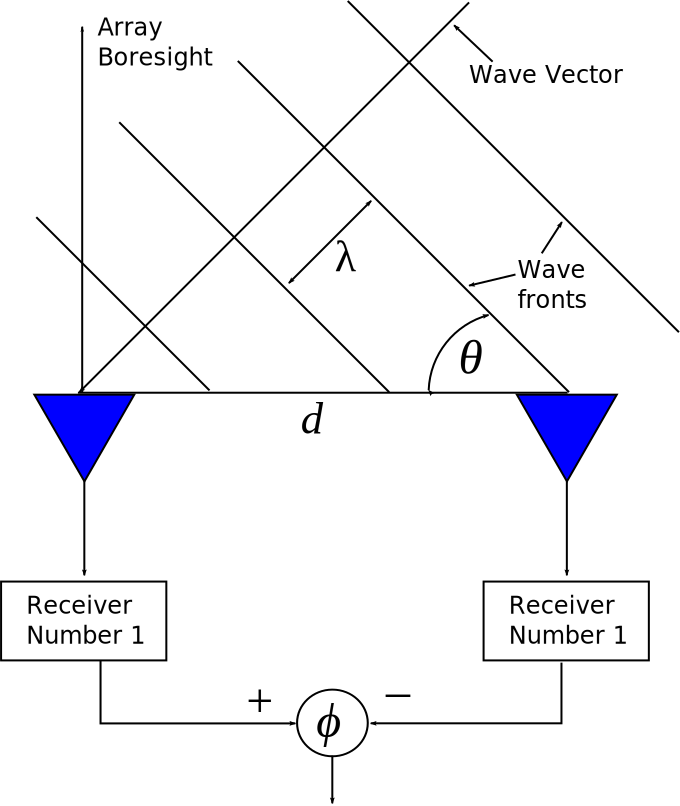
\includegraphics[width=0.4\textwidth]{lit_review/two_element_phase_df_model.pdf}
   \caption{Two-element phase interferometry. Note that as the element spacing (d) is more than half a wavelength there is ambiguity.}
   \label{fig:lit-two-element-phase}
\end{figure}

There are generally three subclasses of phase interferometry systems\cite{jenkins1991smallaperture}:
\begin{description}
  \item [Continuous phase measurement:] A single receiver takes in all of the antenna signals and compares the instantaneous phase of the signals, typically using analogue multipliers. It's fast and relatively simple for two antennas, but becomes complex as the number of elements increases and hence typically has a limited field of view, is susceptible to interference and is not very accurate.
  \item [Phase scanning correlation:] Here, a phase shifter and correlator are used. The phase shifter is varied until the correlator produces a peak output. Again, this is simple for two antennas but becomes complex when multiple phase shifters need to be varied. It is also slow as the phase shift needs to be swept to find the peak correlator output.
  \item [Fourier transform method:] The received signals are digitised and converted to frequency domain, where phase difference measurements are easily taken. As this is a digital technique, spectral processing can be done providing 20 dB to 30 dB of additional sensitivity over the other techniques. Also, working with digital signals in the frequency domain means that phase errors in the signal path can easily be compensated for and adjacent frequency signals can be ignored.
\end{description}
Should the antenna array contain more that two elements, the system either needs to switch between pairs of antennas if it wants to maintain a simple two-input receiver, or it needs a more advanced receiver to sample all antennas simultaneously. The Fourier transform method is the easiest to extend to having more antenna inputs, as the computation is done in the digital domain. Having all antennas processed by the receiver simultaneously allows for a faster system as no switching is required and also provides better performance as it can average multiple inputs at once. However, more inputs requires more computation and algorithmic complexity.

\section{Subspace and Statistical Techniques}
This class of techniques attempts to perform eigen analysis, decomposing the spectral or covariance matrix into eigen subspaces for noise and subspaces for signal. In some sense this equates to a beamforming algorithm which attempts to find an angle resulting in the strongest signal. 
Statistical methods generally involve taking snapshots of the signals received at each sensor, \(\vec{r}(t)\) and then calculating the covariance matrix of the received data\cite{poisel2012electronic}.

The advantage of working with multiple subspaces for each signal is that it allows direction finding to take place when there are multiple overlapping signals arriving at the array. Assume there are \(D\) narrow band signal all with unknown AoA parameter arriving at an \(M\) element array in the presence of uncorrelated noise, the problem space can be reduced from \(M\)-dimensional to \(D\)-dimensional\cite{van2004detection}.

It can be shown that the covariance matrix is diagonal for incoherent sources, non-diagonal and non-singular\footnote{A singular matrix is one which is not invertible, meaning the determinant is 0} for partially coherent sources and non-diagonal and singular if at least one of the sources are coherent\cite{poisel2012electronic}. 

Examples of these techniques include\cite{van2004detection}:
\begin{itemize}
  \item Spectral MuSiC (Multiple Signal Classification) which gets multiple signal snapshots to produce an estimated spectral matrix, \(\hat{\mathbf{S}}_{\mathbf{x}}\) and requires knowing the antenna array manifold vector. It can be applied to arbitrary arrays and performs best when the received signals are uncorrelated. The technique does not work when receiving multiple coherent signals.
  \item Root MuSiC, which is a special form of MuSiC allowing simplified polynomial equations provided linear arrays are used, and requires a lower antenna SNR than Spectral MuSiC.
  \item Least Squares and Total Least Squares ESPRIT (Estimation of Signal Parameter via Rotational Invariance Techniques) which constructs identical subarrays from uniform linear arrays, exploiting shift invariance properties of the array. It can be shown that the signal subspace eigenvectors are linear combinations of the array manifold vector. The RMS error for these techniques can be very close to the Cramer-Rao bound for estimation error\cite{van2004detection}.
\end{itemize}
These subspace techniques typically requires knowledge of the number of unique signals, \(D\), being received as they depend on being able to construct \(D\) subspaces. Seeing as coherent signals degrade performance, they suffer from multipath interference.

\section{Radiometer}
A radiometer is a device which is able to provide a very high accuracy approximation of noise power by averaging a large number of noise samples over a long time period. Due to the high accuracy measurements it can make, it is able to detect small changes in received power. 
It does this by achieving a high sensitivity. Sensitivity is the measure of how weak a signal and instrument is able to detect.

We will define power in terms of a matched load heated to a certain temperature observed over a certain bandwidth.
\begin{equation}
  P = kTB
\end{equation}
where \(k \approxeq \SI{1.38e-23}{\joule\per\kelvin}\), the Boltzmann constant. 

System temperature is a combination of noise powers from atmospheric emissions, the warm earth, the cosmic microwave background, receiver noise figure, losses in the RF chain and others. These noise sources mask the RFI signal which we are trying to locate. While typically an RFI signal below the noise floor would not be an issue, in the case of a radio astronomy reserver that signal will in all likelihood still be a problem because the noise floor of the MeerKAT array is so much lower than the RFI DF instrument. In essence, a signal which will be very loud to the telescope may be difficult for the DF system to even detect. Effort will hence need to go into ensuring that this instrument being designed will be able to see signals below its own noise floor. 

As the noise at an antenna is a combination of a multitude of noise sources, the central limit theorem states that output of the antenna will be approximately a normal (Gaussian) distribution. 

The noise temperature is defined as the noise power per unit bandwidth over the Boltzmann constant:
\begin{equation}
  T_N = \frac{P_v}{k}
\end{equation}

Assuming the power of a noise source remains constant, a single sample of the noise source has an RMS error of approximately \(\sqrt{2}T_{sys}\). However, by integrating the noise power from a certain bandwidth \(\Delta B\) over some integration time \(\tau\) the error can be significantly reduced to
\begin{equation}
  \sigma_{T} = \frac{\sqrt{2}T_{sys}}{\sqrt{2B\tau}} = \frac{T_{sys}}{\sqrt{B \tau}}
\end{equation}
Where \(\sigma_{T}\) is the RMS error in the measurement of the noise temperature, \(T\), and \(T_{sys}\) is the actual system noise temperature. Note that \(2B\tau\) is the number of samples acquired

This process used in a radiometer of acertaining a high accuracy approximation of a received signal by integrating the signal over some observation period can also be used in the context of a direction finding system. For this application, a long observation period may be used to extract a weak signal which is burried in noise so that the weak signal may be processed.

\begin{equation}
  \frac{S}{N} = \frac{S}{N}\sqrt{B\tau}
\end{equation}

Tsys = Tsky + Trx where Tsky is thestuff above and Trx is Johnson noise from electronic components. Tsky can't do anything about. Trx lowered by cooling components. 
The Trx is as a result of the Johnson-Nyquist noise. 

Extension to interferometry:

\(SEFD / (N(N-1))/2 \tau 2B)\)

Sources: \url{https://casper.berkeley.edu/astrobaki/index.php/Radiometer_Equation}
\url{https://casper.berkeley.edu/astrobaki/index.php/Radiometer_Equation_Applied_to_Telescopes}
\url{https://www.cv.nrao.edu/course/astr534/Radiometers.html}


\chapter{System Design}
\label{ch:system-design}

This section will contain an abstracted view of the system, with blocks for antanna array, RF front end, digitisers, first stage DSP on ROACH, 2nd stage DSP on PC with ethernet link.

A brief explanation of the design considerations for each stage of the system. Stating that each block will be designed and expanded on in the following chapters.

\include{./tex/40-df-algorithms}
\chapter{RF Front End}
\label{ch:rf-front-end}
\setsvg{svgpath=./img/rf-front-end/}
\graphicspath{{./img/rf-front-end/}}

This chapter details the design and characterisation of the chain of antenna, low noise amplifier (LNA), lower pass filters and cabling. The cabling is important as each RF chain needs to have exactly\footnote{Some phase difference between the RF chains can and will be calibrated out, but the calibration routine is most robust when the RF chain phases are already closely matches} the same phase delay.



\section{Antenna Array}

Some antennas.

\begin{figure}
  \begin{subfigure}{\textwidth}
    \centering
    \includegraphics[width=0.85\textwidth]{antenna-array-on-roof}
  \end{subfigure}\\[1em]
  \begin{subfigure}{\textwidth}
    \centering
    \includegraphics[width=0.85\textwidth]{antenna-s11}
  \end{subfigure}
  \caption{Array of four FD-250 folded dipoles being measured and the result of the S11 measurements showing acceptable performance between \SI{200}{\mega\hertz} and \SI{300}{\mega\hertz}.}
\end{figure}

\section{LNA and LPF Measurements}
As discussed in lit review, Schleher, it is necessary for an interferometry system to have its RF front end components matched. The front end of this system comprises an antenna, a cable from the antenna to a anti aliasing filter, the filter is plugged into an LNA and a cable runs from the LNA to the digitiser. 
It's fairly strightforward to ensure phase matching between cables. Provided the cables are of the same type, their velocity factors will be equal and it is hence only necessary to ensure that they are of the same length.
The LPFs and LNAs however may have phase mismatches due to manufacturing tolerances. 
There are two areas of interest:
\begin{enumerate}
  \item Does the LPF and LNA provide sufficient attenuation above the Nyquist frequency to ensure that no aliasing occurs?
  \item Hope closely are the phases of the sets of LPFs and LNAs matched to each other?
\end{enumerate}

\section{Anti Aliasing}
As per (cite ADC datasheet and show graph here) the iADC is not receptive to signals above 3 GHz. Hence, it is only necessary to ensure that the LPF and LNA have sufficient attenuation from Nyquist frequency to 3 GHz. 

\begin{figure}
  \centering
  \begin{subfigure}{\textwidth}
    \centering
    \includegraphics[width=0.95\textwidth]{zfl500-10-3000}
    \caption{Gain from 0 to \SI{3}{\giga\hertz} in dB. Antialisaing is sufficient}
  \end{subfigure}\\[1em]
  \begin{subfigure}{\textwidth}
    \centering
    \includegraphics[width=0.95\textwidth]{zfl500-10_500-mag-db}
    \caption{Gain from 0 to \SI{500}{\mega\hertz} in dB. Useable seems to be up to \SI{350}{\mega\hertz}}
  \end{subfigure}
  \caption{VNA measurements of S21 of RF chains showing antialising properties}
\end{figure}
\begin{figure}
  \centering
  \includegraphics[width=\textwidth]{zfl500-10-500-phase}
  \caption{Phase from 0 to \SI{500}{\mega\hertz} showing very good phase matching over operating frequency range (below \SI{350}{\mega\hertz}}
\end{figure}

Phase RMS errors (degrees)
0x1: 0.58
0x2 0.64
0x3: 2.3

\input{./tex/57-portable-design}
\section{System Temperature Calculations}
Tsys.
Channel bandwidth = 390 kHz. 
Noise figure: 3.9 dB. 
LNA gain: 20 dB
LPF insertion loss: 1 dB
connector and cable losses: 2 dB


\chapter{Firmware Design}

Here are the steps which were done to produce the hardware for testing purposes.
Discussion emphasis is on what I changed or modified. Blocks which were already in existance are discussed in less detail.

\section{Software Setup}
CentOS which is the open source version of RHEL. Computer with at least \SI{8}{\giga\byte} of memory as the compile process is memory intensive. 
Number of CPU cores is not important as the Xilinx compile process only runs single threaded.
Xilinx SysGen 14.7.
MATLAB R2012B. 
Casp

\section{ADCs}
The ADCs which were available for use were the CASPER iADCs. 
These are 8-bit, dual core ADCs, where each core runs at \SI{800}{\mega\hertz}. The cores can either be interleaved to sample a single antenna at \SI{1600}{\mega\hertz} or 2 antennas at \SI{800}{\mega\hertz} each.

\section{Polyphase Filter Bank}
Consists of a polyphase FIR filter which applies a window to the input signal in order to prevent spectral leakage followed by a FFT block. FFT consumes most resources and thus some optimisations had to be done to it. 4K PFB. FFT was a real FFT block meaning it only outputs the upper half spectrum as the lower half is the same due to input signals being real. 

Shifting schedule set by software. Bit growth occurs at each stage. If the output of a stage is not shifted down by 1, it risks overflowing. However, if shifting is done unnecessarily, dynamic range is reduced as lower bits are thrown away. Algorithm coded to find optimal shifting. Discuss algorithm here.

\section{Cross Multiplier}
After the FFT, each antenna combination is multiplied together, one being the original signal and one being the complex conjugate. This is somewhat equivalent to dividing the complex numbers, where the key output is that the phase difference between the two antennas is produces. Some maths here to show that this is true. 

Optimisations done here: these are fairly large multiplier. Each pair of antennas requires an 18 bit multiplier for the real and imag components, for both simultanious channels. This means 4 18-bit multipliers for 10 combinations. 40 x 18-bit multipliers is a lot of hardware! 
To mitigate this, I made a change to the complex multiplier block to allow selecting of DSP48E for multipliers. This change was committed back into the centeral code repo for all to use.

Output of a 18\_17 x 18\_17 is a 37\_34. 

\section{Vector Accumulator}
The output vector (2K complex elements) is accumulated by summing each element. 
This is accumulated to a 48 bit number, hence allowing for substantial growth. 
This is key to getting a very good phase difference approximation as uncorrelated noise is integrated out. 
The vector accumulator is implemented by two DSP48E blocks, one for the real and one for the imag components. 
This is followed by a bram which stores and feeds back the vector to the DSP48E adder. 

The design is such that 48 bits are continuously accumulated. After the accumulation has run for a configurable number of iterations, the most significant 32 bits are sliced off and snapped. By accumulating 48 bits, no data is thrown away until the snap. Commit XXXXX makes this change to the dsp48\_bram\_vacc block in the casper library.


\chapter{Software Interface}
\label{ch:software-design}

\section{Code Structure}
It was necessary to write code to allow the computer to interface with the correlator running on the ROACH.
The code had to be carefully designed in accordance with good object orientated design methodologies in order to provide a useful, well defined and easily extendible interface to other code which needs to interface with the correlator.
As such, there was significant emphasis encapsulating logic into classes which mirrored the physical structure of the correlator in the sense of modularising the key components and writing reusable code.
Following is a discussion of the software interface to the correlator with specific focus on the various classes and interfaces.

Instance of a correlator is created.
This then includes:
\begin{enumerate}
  \item An instance of a ControlRegister
  \item Multiple instances of Snapshot classes. One will be created for each snapshot block on the FPGA.
  \item Multiple instance of the Correlation clas, one for each of the cross correlation baselines.
\end{enumerate}

The direction finder code takes an instance of a correlator which can then be used for easy access to the data from the orrelator.

\subsection{Control Register}
The control register naturally lends itself to a class with interfaces to modify the different bit groups of the register in logical ways.
A python module called software\_register was written with a single class: ControlRegister. This class contains a value parameter which mirrors the value programmed into the FPGA's control register. It then has the following interface methods:
\begin{description}
  \item[pulse\_sync] Toggles the syncronisation reset bit low to high and then high to low.
  \item[block\_trigger ; allow\_trigger] These methods either set of clear bit the bit that controls the gate which blocks or allows the snapshot blocks being triggered by a complete accumulation. The idea is that this will be used to allow all of the snapshot blocks to be armed sequentially before they can be triggered all at once.
  \item[reset\_accumulation\_counter] Pulses the bit which resets the counter which increments every time an accumulation completes and triggers the snap blocks. This counter lets us keep track of how many accumulations have been performed by the system.
  \item[pulse\_overflow\_rst] Similar to the above, except this clears the latch which gets latched high whenever the FFT block overflows. This essentially allows us to 'acknowledge' that we have seen the occurrence of the overflow flag.
  \item[select\_adc] Controls which of the four RF inputs is connected to the time domain snapshot block via a multiplexer. By multiplexing the steams, it saves the logic and BRAM of having to have four seperate snap blocks, at the expense of one multiplexer and not being able to synchronously sample the ADC streams in the time domain. This is considered an acceptable tradeoff due to the fact that the time domain snap is only designed to be used for getting an approximation of the signal strength arriving at an antenna and this does not need to be done in parallel for each antenna.
  \item[set\_shift\_schedule] This methods takes a \SI{12}{\bit} number and sets the FFT shift schedule to that number. While this design only has a 10 stage FFT, 12 bits is kept in the register for future expansions.
\end{description}

All of the methods in this class log their actions as well as the new value of the control register when it is modified at the debug log level.

\section{Calibration}


The software needs to have provision to calibrate various aspects:
\begin{itemize}
  \item RF front end: the LPF and LNA and cable from LNA to ROACH may have different delay or phase shift factors. Measurements in earlier chapters show not really different, but worth doing any way for future systems which may have RF front ends with more significant shifts. This can be calibrated very accurately using a known signal though the RF chain and measuring the response.
  \item Same as above but in time domain
  \item Antenna cables: the antennas which were purchased for this project do not have the same length cables. Table (following) shows various lengths. It would be difficult to imperically measure the phase shift caused by these cables. Rather, by knowing the velocity factor through the cable and measuring the length of the cable the difference can be deduced.
\end{itemize}

\subsection{Antenna Cable Length Compensation}
\begin{table}
  \centering
  \begin{tabu}{c|c}
    Antenna Number & Cable Length (m)\\
    \hline
    0 & 0.557 \\
    1 & 0.566 \\
    2 & 0.510 \\
    3 & 0.590
  \end{tabu}
  \caption{Lengths of cables coming out of antennas}
  \label{tab:software-antenna-cable-lengths}
\end{table}

According to the manufacturer, Magnavolt, the cables are all RG214 which has a velocity factor of 0.659. 

Wrote JSON file with this information.

For each baseline, software calculates difference in propagation times for each element of the baseline created by length and velocity factor. Calculates corresponding phase shift for each frequency bin based on this and then aplies this frequency shift to the cross correlation in there.

Here: extract of JSON file.
A bit of maths of what the software does?

Discuss how this applies to both time and frequency domain.

Two cables: \SI{0.512}{\meter} and \SI{1.005}{\meter}. Both RG58. According to datasheet, velocity factor of 0.66.
Theoretical delay:
\begin{equation}
  \begin{split}
    t &= \frac{l}{\text{vf} \times c}\\[1em]
  \therefore \Delta t &= \frac{l_a}{\text{vf}_a \times c} - \frac{l_b}{\text{vf}_b \times c} \\[1em]
                      &= \frac{1.005}{0.66c} - \frac{0.512}{0.66c} \\[1em]
    &= 2.4899 \text{ ns}
  \end{split}
\end{equation}
VNA shows Propagation delay difference of \(\frac{5.2532+5.1916}{2} - \frac{2.7443+2.7206}{2} = 2.4901\) ns. This is a difference of below \SI{0.1}{\percent}.

\begin{table}
  \centering
  \begin{tabu}{c|r|r}
    Visibility & Uncompensated (ns)& Compensated (ns)\\
    \hline
    0x1 & 2.492 & 0.002 \\
    0x2 & 2.489 & -0.002 \\
    0x3 & 2.495 & 0.002 \\
    1x2 & -0.001 & -0.002 \\
    1x3 & 0.001  & 0.000 \\
    2x3 & 0.005 & 0.005
  \end{tabu}
  \caption{ADC sample period: \SI{1.25}{\nano\second}. Upsampled correlation step size: \SI{1}{\pico\second}}
  \label{tab:software-cable-lenth-compensation}
\end{table}

It's clear that the system is able to correctly measure the cable length difference to within \SI{3}{\pico\second} accuracy which is below 1 hundredth of the ADC sample period.
Also it's clear that the system can successfully apply the calibration factors from the JSON file specifying cable length and velocity factor and compensate for the cable length mismatch down to the same level of accuracy: below 1 hundredth of an ADC sample.

\begin{figure}
  \centering
  \includegraphics[width=0.9\textwidth]{two-cables-vna}
  \caption{Two different length cables on VNA doing time measurement showing propagation delay difference of \SI{2.49}{\nano\second}}
  \label{fig:software-two-cables-vna}
\end{figure}


\subsection{RF Chain Compensation (Calibration?) in Frequency Domain}
The LPF + LNA + Long RG58 cable from the front end to the roach introduces difference phase and time shifts. 

\begin{figure}
  \centering
  \begin{subfigure}[b]{0.49\textwidth}
    \centering
    \includegraphics[width=0.95\textwidth]{freq-shift-full-rf-chain}
    % left, bottom, right, top
    \caption{Phases before calibration}
  \end{subfigure}
  \begin{subfigure}[b]{0.49\textwidth}
    \centering
    \includegraphics[width=0.95\textwidth]{freq-shift-full-rf-chain-after-cal}
    % left, bottom, right, top
    \caption{After cal}
  \end{subfigure}
  \caption{Bar}
\end{figure}

\subsection{RF Chain Compensation in Time Domain}

\begin{figure}
  \centering
  \begin{subfigure}[b]{0.49\textwidth}
    \centering
    \includegraphics[width=0.95\textwidth]{time-delay-through-full-rf-chain}
    % left, bottom, right, top
    \caption{Phases before calibration}
  \end{subfigure}
  \begin{subfigure}[b]{0.49\textwidth}
    \centering
    \includegraphics[width=0.95\textwidth]{time-delay-in-phase}
    % left, bottom, right, top
    \caption{THIS IS WRONG. GENERATE AND USE CALIBRATED IMAGE HERE.}
  \end{subfigure}
  \caption{Bar}
\end{figure}

\input{./tex/75-software-array-coordinate-calculator}
\section{Frequency Domain Direction Finding}
For weak, narrow band, continuous signals.
Foo.

\section{Time Domain Direction Finding}

\subsection{Testing}
Measure propagation delay of cables on VNA. Screenshot.
Put same cables onto system and look at delay according to system. 
Profit.

\subsection{Upsampling}
Use the word 'interpolate' somewhere...
Can upsample. Why? Band limited signal sampled above Shannon/Nyquist sampling requirement. Hence we have all possibe information. Hence we're allowed to interpolate as much as is wanted. 
Want to upsample to provide better resolution. Note accuracy does not go up, it's dependant on sample rate, jitter, ENOB etc. But resolution can be arbitrarily increased by upsampling.

Two ways. More intuative: upsample signal then cross correlate. 
Or cross correlate then upsample. Second is FAR more efficient computationally. 
Time is faily linear with x then upsample. Time is very dependant on signal length with first. Assume it has to do with resample being based on FFT and FFT performing differently with different signal lengths. With x then upsample, signal lenght to be upsampled known before hand.
Upsample then X much more expensive as it needs to upsample the full signal and then X on the huge resulting signal.
X first does only a few steps of X, producing only a few output vectors then upsamples each of those.

Resample first:
Depending on signal length which is controlled by length of pulse, not deterministic, the FFT is \(\Omega(N\log{N})\) to \(\mathcal{O}(N^2)\). Next stage, cross correlation does a whole lot of point MACs. \(\mathcal{O}(N)\). This is dominated by the resample phase. 

X first: Does \(\mathcal{O}(N)\) MACS. Result is a small output vector. Not dependant on N. Hence the resample stage becomes \(\mathcal{O}(1)\). 

Perhaps look at this again for N being the amount of upsampling being done rather than signal length. Or amount of padding?

Table: Variable: (sig len, upsampling, padding). Best case O. Worst case O. 

A few pictures here:
Non upsampled and upsampled correlation.
\begin{figure}
  \centering
  \begin{subfigure}[b]{0.49\textwidth}
    \centering
    \includegraphics[width=\textwidth]{software/noise-no-upsampled}
    \caption{a}
  \end{subfigure}
  \begin{subfigure}[b]{0.49\textwidth}
    \centering
    \includegraphics[width=0.92\textwidth]{software/noise-with-upsampled}
    \caption{b}
  \end{subfigure}
  \caption{Bar}
\end{figure}

\begin{figure}
  \centering
  \includegraphics[width=\textwidth]{software/time-domain-cross-raw-vs-upped}
  \caption{Bar}
  \label{fig:software-aseaweawea}
\end{figure}

\begin{figure}
  \centering
  \begin{subfigure}[b]{0.49\textwidth}
    \centering
    \includegraphics[width=0.95\textwidth]{software/time-delay-through-full-rf-chain}
    % left, bottom, right, top
    \caption{Phases before calibration}
  \end{subfigure}
  \begin{subfigure}[b]{0.49\textwidth}
    \centering
    \includegraphics[width=0.95\textwidth]{software/time-delay-in-phase}
    % left, bottom, right, top
    \caption{THIS IS WRONG. GENERATE AND USE CALIBRATED IMAGE HERE.}
  \end{subfigure}
  \caption{Bar}
\end{figure}

\subsection{Calibration}
Different RF chains may have different propagation delays. 
Inject broad band signal into each baseline. Should be zero delay between each. 
If delay is non-zero, write it to calibration file.
For future measurements, subtract this calibration offset from measured delay. 

Here: image of cross correlations of all pre-cal baselines. Single plot. Use long signals for high and narrow peak.
There is another cal section. Merge?

\subsection{De-dispersion}
We're assuming constant propogation delay across frequency. VNA shows mostly correct, but not perfectly. Also other systems have have different dispersion factors. 
De-dispersion. 
More difficult but: single set of coefficients would be used from both time and frequency systems. 
Need a perfect pulse.
Would be very useful to following systems which use the pulses for RFI classification. 
For now: folded dipole antennas should provide minimal dispursion. 
VNA measurements shows cables not very dispersive.

\input{./tex/78-software-logging.tex}

\chapter{User Interface}
\label{ch:user-interface}

The UI is modeled on that presented in \cite{guerin2012passive}.


\chapter{Field Trials}
\label{ch:field-trials}

\section{Power supply}
It was necessary to power the ROACH from a battery in order to allow it to be portable and taken out into the open field.
Initially the plan was to power it from an inverter running off of a battery. Here, discuss why the inverter may be too noisy. Can this be shown from reverb chamber measurements?

Instead, an ATX power supply which runs directly from a \SI{12}{\volt} battery was made available from the SKA equipment. The power supply is made by Mini-Box and its part number is PicoPSU-80-WI-32V. This can output \SI{80}{\watt} which is enough to run the ROACH. To connect it, the traditional mains-powered ATX powersupply is disconnected from the motherboard and this module is plugged into the motherboard. This is shown in (insert figure here!).

Furthermore, a ROYAL 1150K battery was supplied. This is a \SI{105}{\ampere\hour} deep cycle calcium battery.
As the ROACH draws X amps at \SI{12}{\volt}, this implies that we are discharging the battery at \(\frac{105}{X} = \frac{C}{Y}\).
It is advised to not run down below \SI{70}{\percent} to maintain the battery lifespan. As shown by (cite battery charging), this implies that the voltage should not drop to below \SI{12.1}{\volt} when discharging at \(\frac{C}{Y}\)

Testing in the lab showed that the ROACH pulled \SI{3.1}{\ampere} at \SI{12}{\volt} which is \SI{37}{\watt}. This can easily be handled by the \SI{80}{\watt} ATX power supply. 
Testing by running the ROACH from the battery overnight. The battery started at \SI{12.6}{\volt} and had dropped to \SI{11.9}{\volt} \SI{15}{\hour} later. The purpose of this test was not to provide a comprehensive report of the capacity of the battery or the requirements of the ROACH, but simply to show that the system will easily be able to run for a few hours in the field during field trials.

\section{Signal Source}
The signal source used is a portable HAM radio, lent by Jason Manley of the SKA. 
It's rated output power is \SI{5}{\watt}. Free space path loss equation will be calculated to get an approximation of the power going into the LNAs and the power going into the ADCs. At \SI{2500}{\mega\hertz}, \(\lambda = \SI{1.2}{\meter}\). The maximum gain of the FD-250 folded dipole is approximately \SI{0}{\dBi}.

\begin{align}
  P_r &= P_t G_t G_r \left( \frac{\lambda}{4 \pi R} \right)^2 \\
      &= \SI{5}{\watt} \times 1 \times 1 \left( \frac{\SI{1.2}{\meter}}{4 \pi \times \SI{60}{\meter}} \right)^2 \\
      &= \SI{0.0000127}{\watt} \\
      &= \SI{0.0127}{\milli\watt} \\
     &= \SI{-19}{\dBm}
\end{align}

After the \SI{20}{\decibel} gain of the ZFL-500HLN LNAs, the power into the iADCs is approximately \SI{1}{\dBm}. Seeing as the ADC's full scale range is \SI{0}{\dBm}, a \SI{10}{\decibel} attenuation will be inserted after each LNA to bring the input signal down to a safe level.

\chapter{Conclusions}
\label{ch:conclusions}
\graphicspath{{./img/conclusions/}}
Foobar
That is all.


\appendix
\include{./tex/b0-appendix-roach-dev}
\include{./tex/c0-appendix-adc-cal}
\include{./tex/d0-array-construction}

\bibliographystyle{IEEEtran}
\bibliography{./tex/bib}
\end{document}
